\section{Preliminary Results}
In our preliminary work we have developed AAnchor - a method for locating amino acids in a cryo EM maps of high resolution, and cryo-GAN  - VAE-GAN based simulation of a cryo EM map.
\subsection{cryo-GAN}\label{s:c-GAN}
\subsubsection{Motivation}
While there is a high demand for realistic cryo-EM simulation, the most popular  existing tool (callled  molmap) performs Gaussian Blurring on atoms.

While a synthetic map represents  an "ideal" universe, in an experimental map the noise is not i.i.d gaussian and different regions have different volume density. 
Moreover, it is assumed that some of the physico-chemical properties which affect experimental cryo-EM maps such as charge and atomic bonds, are not captured by the existing simulation. 
Fig. \ref{f:6nt8} shows experimental and "molmap" map of the STING protein (pdb ID 6nt8, \url{https://www.rcsb.org/structure/6NT8}).
\subsubsection{Methods}
A three dimensional VAE-GAN network was used for map generation. The network architecture is shown in Fig. \ref{f:cryo-GAN}. 
The network input is an atomic structure fragment after voxelization, i.e., five (for each atom H, C, O, S, N) 3D matrices (called channels).
The output is a cube of a cryo-EM map - 3D matrix of density.
Due to the normalization implied in the training phase, cryo-GAN generates cubes with mean value 0.5 and standard deviation of 0.16.
The proposed  cryo-GAN architecture differs from the well known image generating  architectures ( \cite{Larsen2016,Wu}) in three aspects:
\begin{itemize}
    \item Input: The input is five channels of 3D matrices, while in \cite{Larsen2016} and \cite{Wu} the input is 2D images.
    \item Reconstruction Loss (RC Loss).
    Traditionally RC loss is the mean square of the difference between the obtained and the reference images.
    We  added mean and standard deviation  terms, i.e., there is a penalty if the mean value or the standard deviation of the created 3D cube differ from the required ones.
    \item Discriminator: The role of a discriminator is to distinguish between real (input) and  fake (generated) map cube. 
    Usually in GANs the output is generated from a random input, sampled from the same distribution. 
    In our case the output is generated from a deterministic input - atomic model fragment,  so we feed the  atomic model fragment to the discriminator in addition to the generated map cube.
\end{itemize}
We implied the training strategy recommended in \cite{Wu}:1) GAN loss  was not backpropagated to the discriminator, 2) discriminator parameters were updated only if its accuracy fails below 80 \%.



\subsubsection{Results}
\textbf{Training phase results} are shown in Fig. \ref{f:gan_res}.
Loss and discriminator convergence show that the network  has converged and is not overfitted.
The \textbf{generated synthethic map } of  STING protein (pdb ID 6nt8) is shown in  Fig. \ref{f:6nt8_newsim}.
While from visual inspection the map resembles the experimental map (see Fig. \ref{f:6nt8_real}),  an additional evaluation criterion is required.
To evaluate the quality of a generated map, an additional discriminator, named \textbf{evaluation discriminator} was trained independently from the cryo-GAN network. 
The evaluation discriminator was trained independently to distinguish  real maps from those created by "molmap" and random data.
Training results of the evaluation discriminator are shown in Fig \ref{f:disc_train}.
Evaluation of the map generated by cryo-GAN is performed by running the evaluation discriminator on each  voxel of the map.
56 \% of the cryo-GAN map voxels were labeled as "real".




\begin{figure}[!ht]
\begin{minipage}[b]{0.45\linewidth}
\begin{subfigure}[b]{\linewidth}
	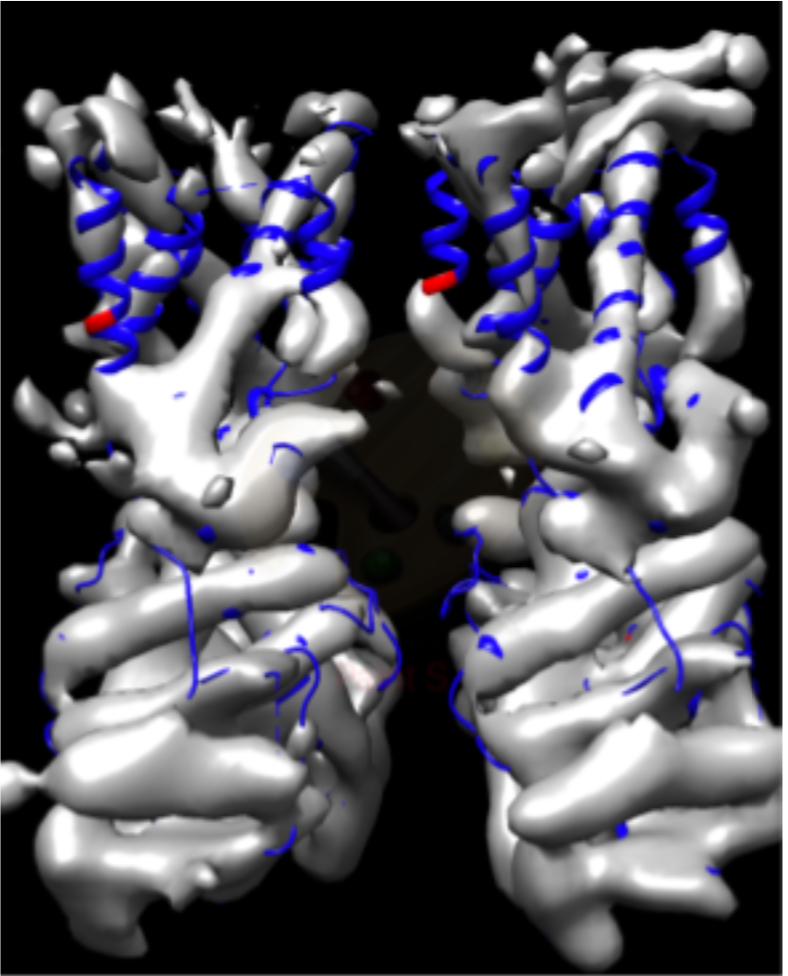
\includegraphics[width=1.0\textwidth]{picsnew/6nt8_real.png}
	\caption{Experimental map of protein 6NT8, EMD-0505}
	\label{f:6nt8_real}
\end{subfigure}
\end{minipage}
\begin{minipage}[b]{0.45\linewidth}
\begin{subfigure}[b]{\linewidth}
	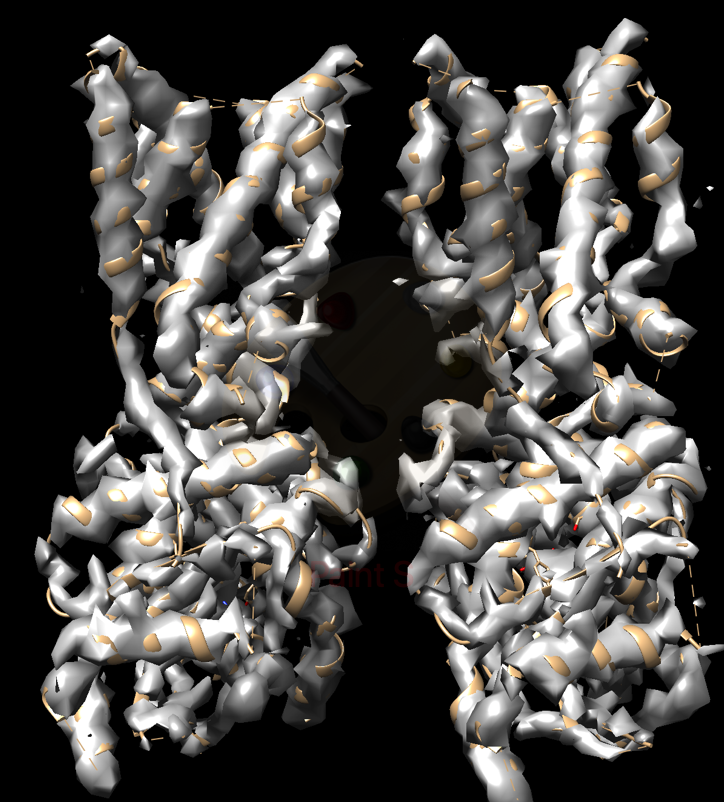
\includegraphics[width=1.0\textwidth]{picsnew/6nt8_molmap.png}
	\caption{Synthetic Map of  protein 6NT8, created using "molmal" command.}
	\label{f:6nt8_molmap}
\end{subfigure}
\end{minipage}
\caption{Cryo EM maps of protein 6NT8: experimental and simulated by molmap }\label{f:6nt8}
\vspace{-3mm}
\end{figure}

\begin{figure}[!ht]
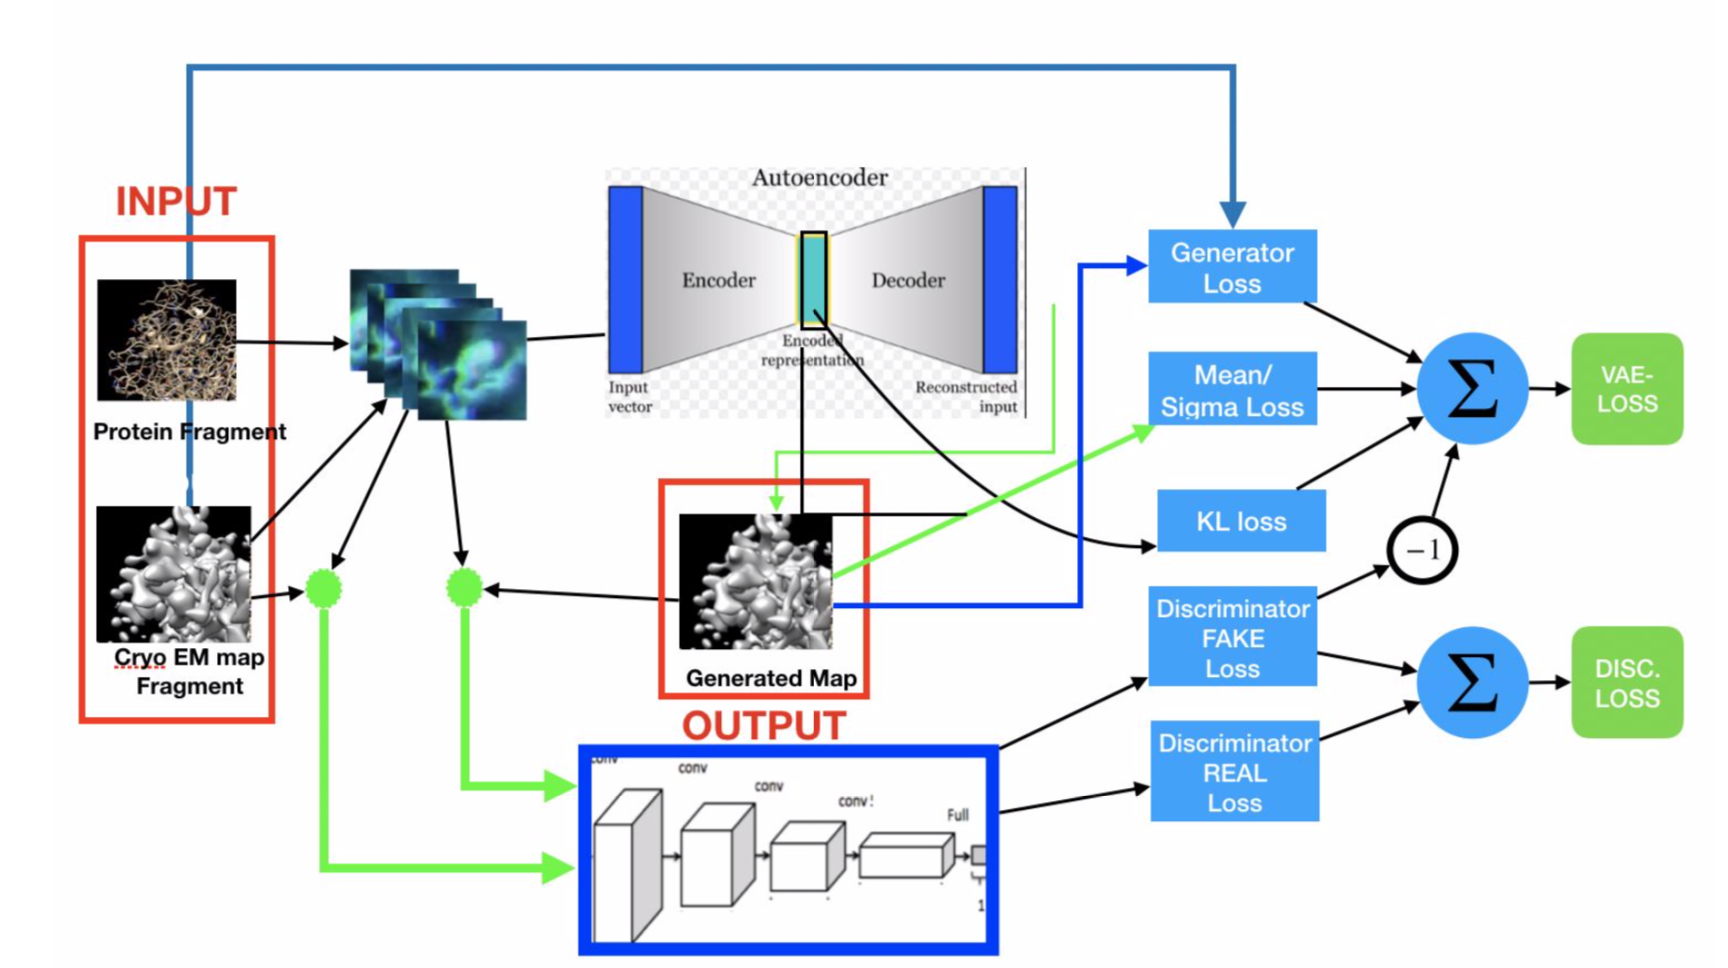
\includegraphics[width=0.95\textwidth]{picsnew/cryo_GAN.png}
\caption{Cryo-GAN architecture.}\label{f:cryo-GAN}
\end{figure}

\begin{figure}[!ht]
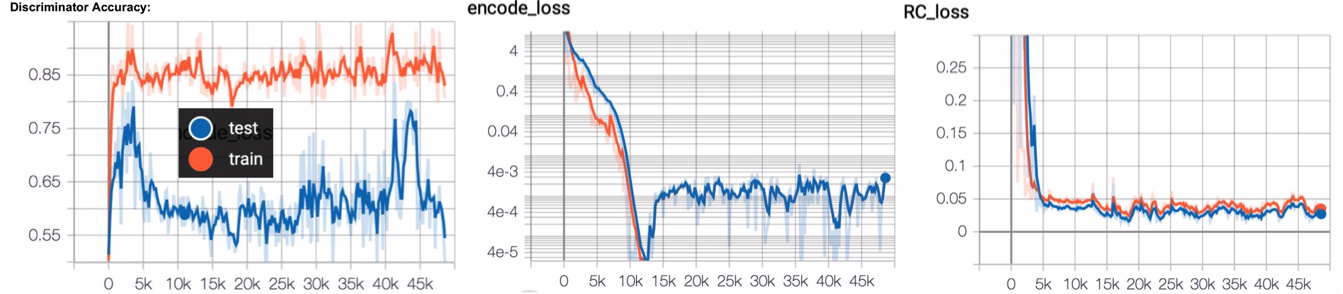
\includegraphics[width=0.95\textwidth]{picsnew/gan_res.png}
\caption{Training Phase Results for Cryo-GAN. Discriminator accuracy on train data of 80 \% agrees with training strategy. Discrimator Accuracy of 50 \% on test data means that the discriminator cannot distinguish between real and synthetic maps. RC loss and Encode loss converge on train and test data, meaning that both the Encoder and the Generator converged}\label{f:gan_res}
\end{figure}

\begin{figure}[!ht]
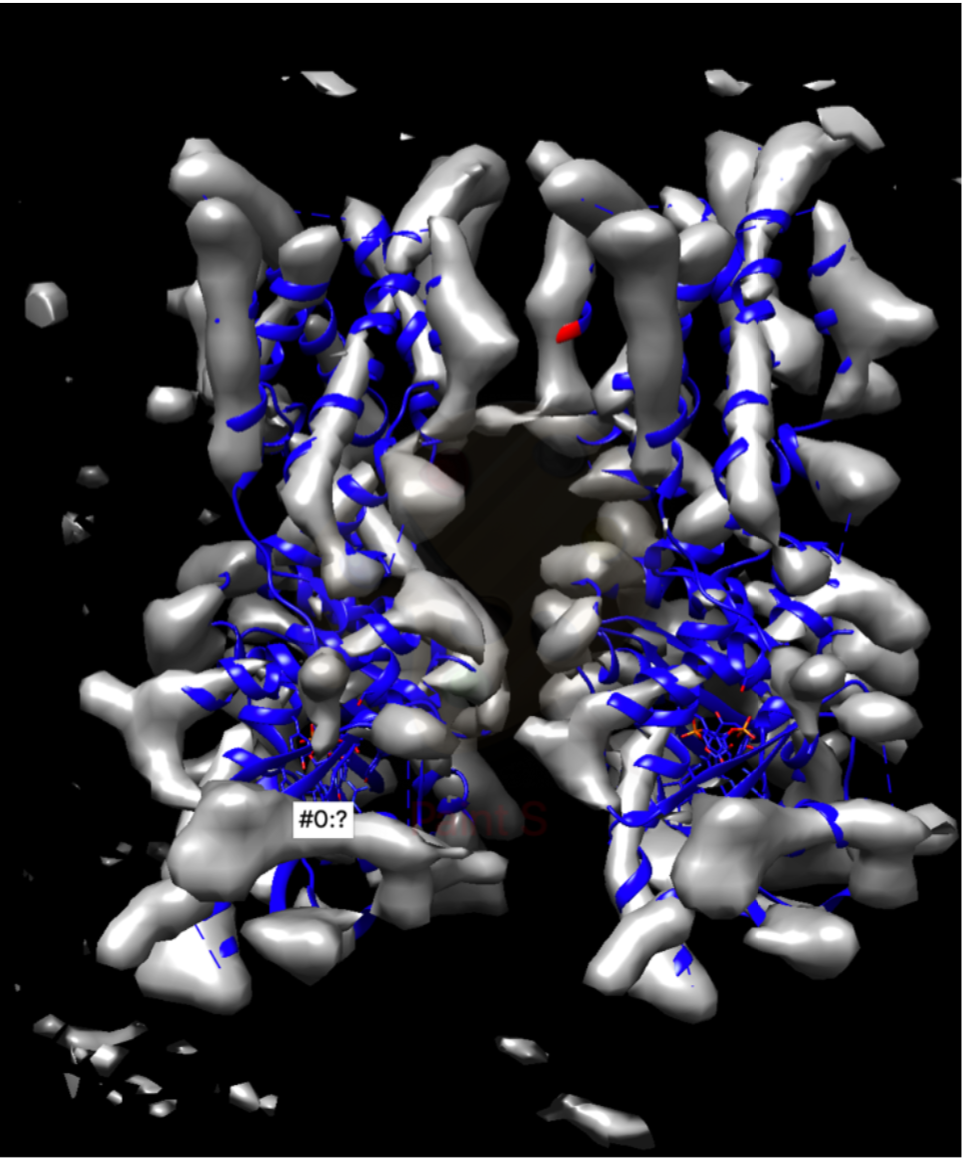
\includegraphics[width=0.95\textwidth]{picsnew/6nt8_newsim.png}
\caption{Genarated map of STING protein (pdb ID 6nt8) }\label{f:6nt8_newsim}
\end{figure}

\begin{figure}[!ht]
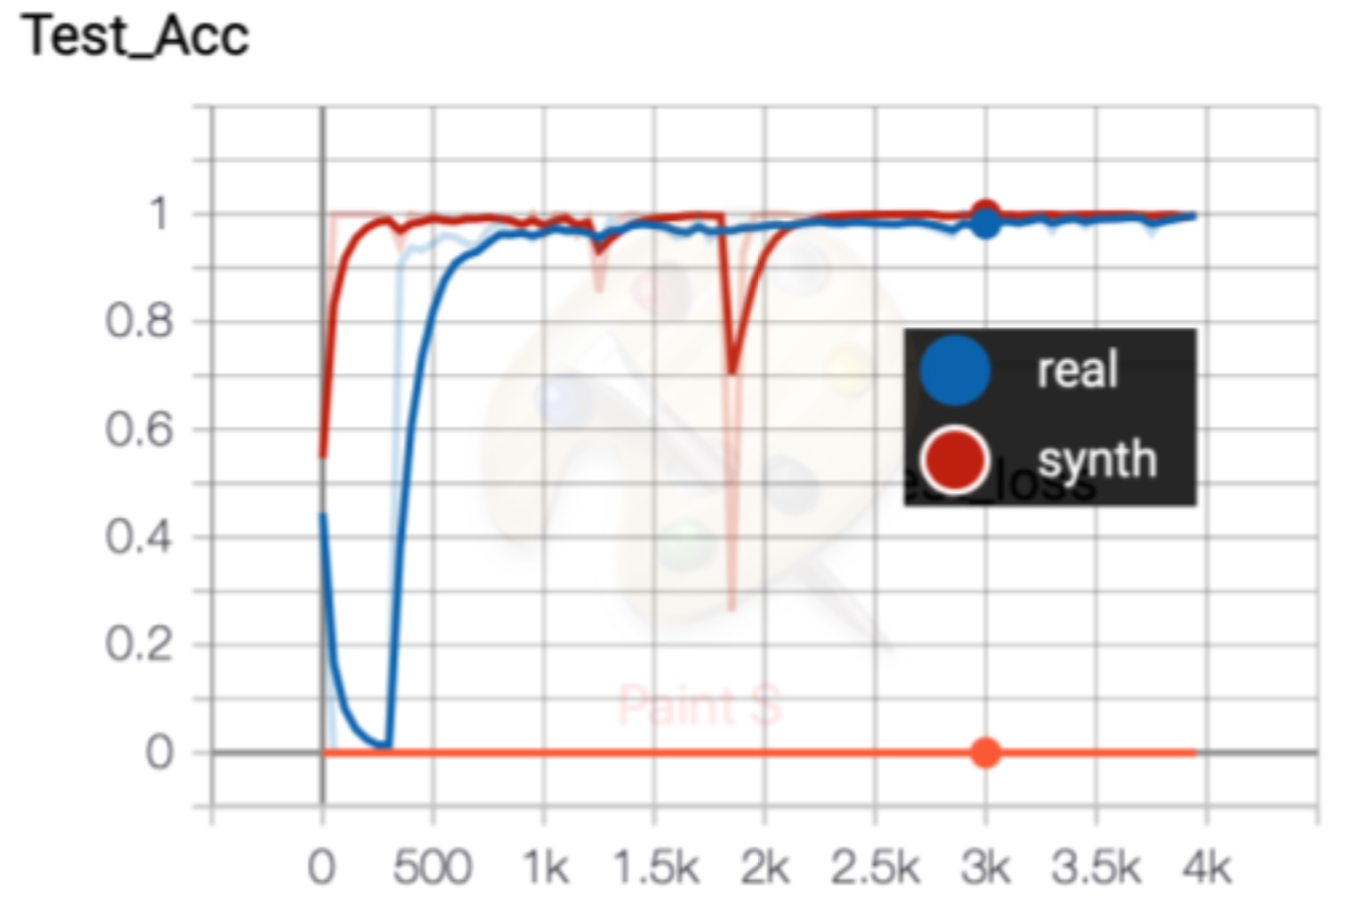
\includegraphics[width=0.95\textwidth]{picsnew/dicc_train.png}
\caption{Training Results of the evaluation discriminator }\label{f:disc_train}
\end{figure}

\subsection{AAnchor}
AAnchor \cite{Rozanov2018AAnchor:Maps} succeeded to detect with confidence of above $80 \%$ a significant percentage of amino acids in  cryo EM maps  of resolutions  of $3 $ {\AA}  and below.
Analysis of the AAnchor detection performance brings to the following observations:
\begin{enumerate}
    \item The CNN Classifier combined with an effective search algorithm is capable of detecting a sufficient number of amino acid "anchors".
    \item The  CNN classifier performance is critical for the amino acid detection performance. Designing and training a high precision classifier is key to a precise detection algorithm.
    \item Synthetic Data can be used to improve classification performance if there is  lack of experimental data.
    \item Appropriate confidence estimation can be obtained from a classification CNN using a simple calibration process.
\end{enumerate}

\subsubsection{AAnchor overview}
Given a cryo EM map at high resolution, 
AAnchor finds the position and type of amino acids within the map.
The method is divided to two main procedures: classification and detection. 
\begin{enumerate}
\item 
The \textbf{classification} problem is defined as the assignment of one out of 21 labels (20 amino acids plus "none") to a voxel and its close neighborhood. An amino acid  is assigned to a voxel if its center of mass is within $1.5$ {\AA}   from the  voxel position.
\item
The \textbf{detection} problem is defined as the localization of amino acids of a specific type in the cryo EM map.
The output of the detection problem are the coordinates of the detected amino acid center of mass followed by estimated confidence.
\end{enumerate}


 Inspired by the similarity of our tasks to the known image processing problems we built a CNN that classifies each voxel to 21 types. 
We  trained and tested this CNN on simulative and experimental cryo EM maps at  resolutions $2.2$ {\AA}  , $2.9$  {\AA} , and $3.1$ {\AA} .
Using the sliding window approach and post-processing filtration, we applied  the trained  classification CNN to the detection problem.

\subsubsection{The Classification CNN performance}

Once trained, the CNN is used to perform prediction on a test dataset, which is disjoint from the training set.
For each input cube with known label $j$, the softmax CNN produces "probabilities" $p_k$, $k=0,\cdots,C$. 
The predicted label $i$ is the one giving maximal "probability", and the confidence is $p_i$.
We show the classification results  by plotting the obtained  \textbf{confusion matrix} ( \cite{Fawcett2006}).

% It is desired that softmax CNN be \textbf{well calibrated} \cite{Guo2017OnNetworks}, i.e., the predicted confidence should reflect the ground truth probability.
% A \textbf{reliability curve} is a plot of ground truth accuracy prediction vs reported confidence. 
% For a perfectly calibrated network the probability curve is an identity function. 
% For the experimental results the ground truth accuracy is estimated by grouping predictions in interval bins according to their reported confidence \cite{Guo2017OnNetworks}. 

\subsubsection{Classification Accuracy}
\paragraph{$2.2$ {\AA}  Resolution.} We have the CNN performance on a 
$2.2$ \AA cryo-EM map of $\beta$-galactosidase \cite{Bartesaghi2015} (EMD-2984).
At the time of the research, only three additional cryoEM maps with resolution better than $2.3$ {\AA}  were available: EMD-8762 \cite{Dong2017},EMD-8194 \cite{Merk2016}, and EMD-3295 \cite{Banerjee2016}.
Even augmented, this is definitely not enough for proper training of the CNN.
The confusion matrix obtained for the  CNN trained on the experimental data is shown in Figure \ref{f:CM_22_RR}.
A much better accuracy is achieved if the experimental data is mixed with the synthetic (simulated) data in the training data set. Figure ~\ref{f:CM_22_RSR} shows the confusion matrix in this case.


\begin{figure}[!ht]

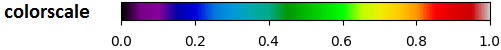
\includegraphics[width=0.45\textwidth]{pics/scale.png}

\begin{minipage}[b]{0.49\linewidth}
\begin{subfigure}[b]{\linewidth}
	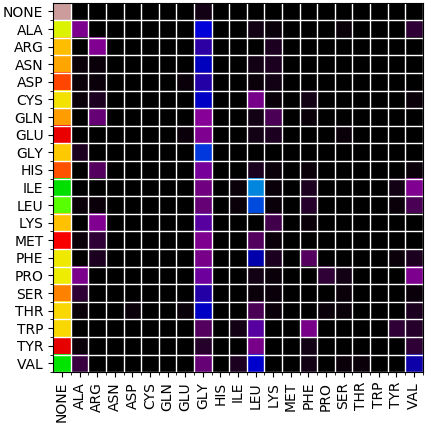
\includegraphics[width=1.\textwidth]{pics/CM_22_RR.png}
	\caption{\scriptsize
	Train: Experimental. \\
	Test :Experimental}
	\label{f:CM_22_RR}
\end{subfigure}
\end{minipage}
\begin{minipage}[b]{0.49\linewidth}
\begin{subfigure}[b]{\linewidth}
	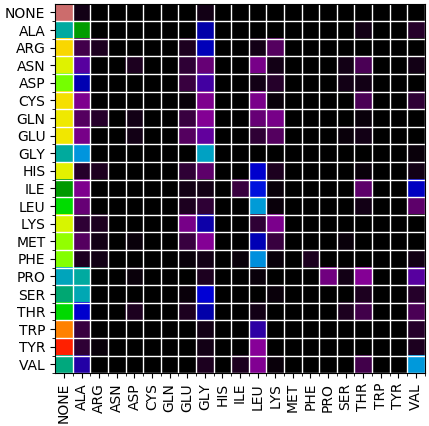
\includegraphics[width=1.\textwidth]{pics/CM_22_RSR.png}
	\caption{\scriptsize
	Train: Sim+Exp. \\
	Test :Experimental}
	\label{f:CM_22_RSR}
\end{subfigure}
\end{minipage}
\caption{Confusion matrix obtain for variuos training sets  for Resolution $2.2 $ {\AA} .
An entry $a_{i,j}$  of a confusion matrix ( \cite{Bartesaghi2015}) $A$ is defined as the ratio  $a_{i,j} = \frac{T_j^j}{N_j}$,  where  $N_j$ is the number of input cubes labeled $j$ and  $T_j^i$ the number of inputs labeled $j$ with predicted label $i$.
}
\vspace{-3mm}
\end{figure}

\paragraph{Resolutions $2.9$ {\AA}  and   $3.1$ {\AA}  }
Coarsening the resolution has two opposite effects on the classification accuracy.
Intuitively, in higher resolution maps the amino acids shape is sharper, however lower resolution maps benefit from a larger training dataset.
The confusion matrices for $2.9$ {\AA}  Anthrax toxin protective antigen pore and $3.1$ {\AA}   Lysenin Pore are presented in Figures ~\ref{f:CM_29_RR} and ~\ref{f:CM_31_RR}, respectively. 

 Accuracies for $2.9$ {\AA}  and $3.1$ {\AA}  are significantly better than those for $2.2$ {\AA} . This is clearly due to the increased training dataset. 
 The only exception is Alanine, which is probably too small to be detected at resolutions coarser than $2.2$ {\AA} .
However, moving from $2.9$ {\AA}  to $3.1$ {\AA}  we see that for the majority of the amino acids the total accuracy values are decreased.
Thus, in this transition the effect of increasing the training dataset size did not compensate for the degradation in map precision.
 
 




\begin{figure}[!ht]
\begin{minipage}[b]{0.45\linewidth}
\begin{subfigure}[b]{\linewidth}
	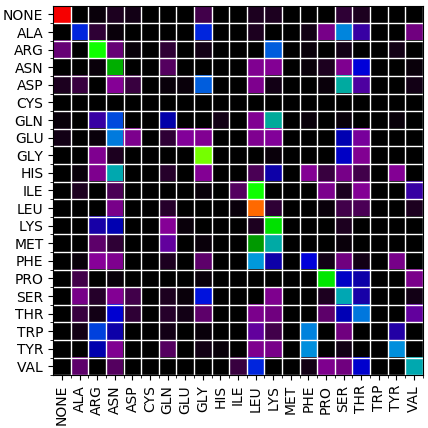
\includegraphics[width=1.0\textwidth]{pics/CM_29_RR}
	\caption{Confusion matrix for $2.9$ {\AA} , test map  EMD-6224}
	\label{f:CM_29_RR}
\end{subfigure}
\end{minipage}
\begin{minipage}[b]{0.45\linewidth}
\begin{subfigure}[b]{\linewidth}
	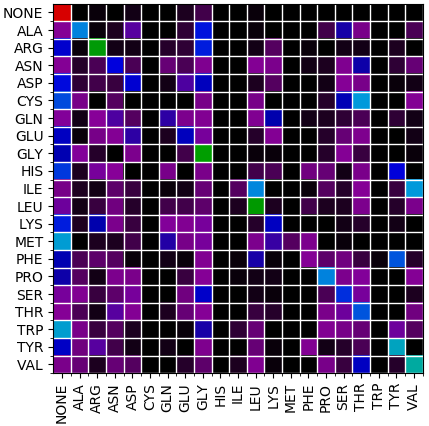
\includegraphics[width=1.0\textwidth]{pics/CM_31_RR.png}
	\caption{Confusion matrix $3.1$ {\AA}  , test map EMD-8015}
	\label{f:CM_31_RR}
\end{subfigure}
\end{minipage}
\caption{Classification Results for Resolution $2.9$ {\AA}   and $3.1$ {\AA} . }
\vspace{-3mm}
\end{figure}

\subsubsection{Detection Results}
Whilst the detection (localization) of all amino acids of a protein seems to be a hard problem at this time, detection of a subset of the amino acids obtained with high confidence is achievable. 
Our goal was to  identify \textbf{anchors}, i.e., amino acids, which have been located and labeled with confidence above $80 \%$. 


% For each resolution case we tested a number of different classification methods, while the pre-processing and post-processing phases remain unchanged.

Table  ~\ref{t31} demonstrates the detection results for various map resolutions.
The fraction of the detected  amino acids is  $10 \%$-$20\%$, depending on resolution.
The best results were achieved for  $2.9$ {\AA}  resolution, where we detected $70 \%$ of prolines.
Recall that all detections contain less than $20 \%$ of errors.
We expect this result to improve, as more high resolution cryo EM maps are being released.

\begin{table}
\small
\begin{tabular}{|m{4cm}|m{4cm}|m{4cm}|}
      \hline
       \Large{ 2.2 {\AA} }: EMD-2984 & \Large{ 2.9 {\AA} }:EMD-6224 & \Large{ 3.1 {\AA} }:EMD-8015\\
      $\beta$ -galactosidase & Anthrax toxin protective antigen pore & Lysenin Pore  \\
      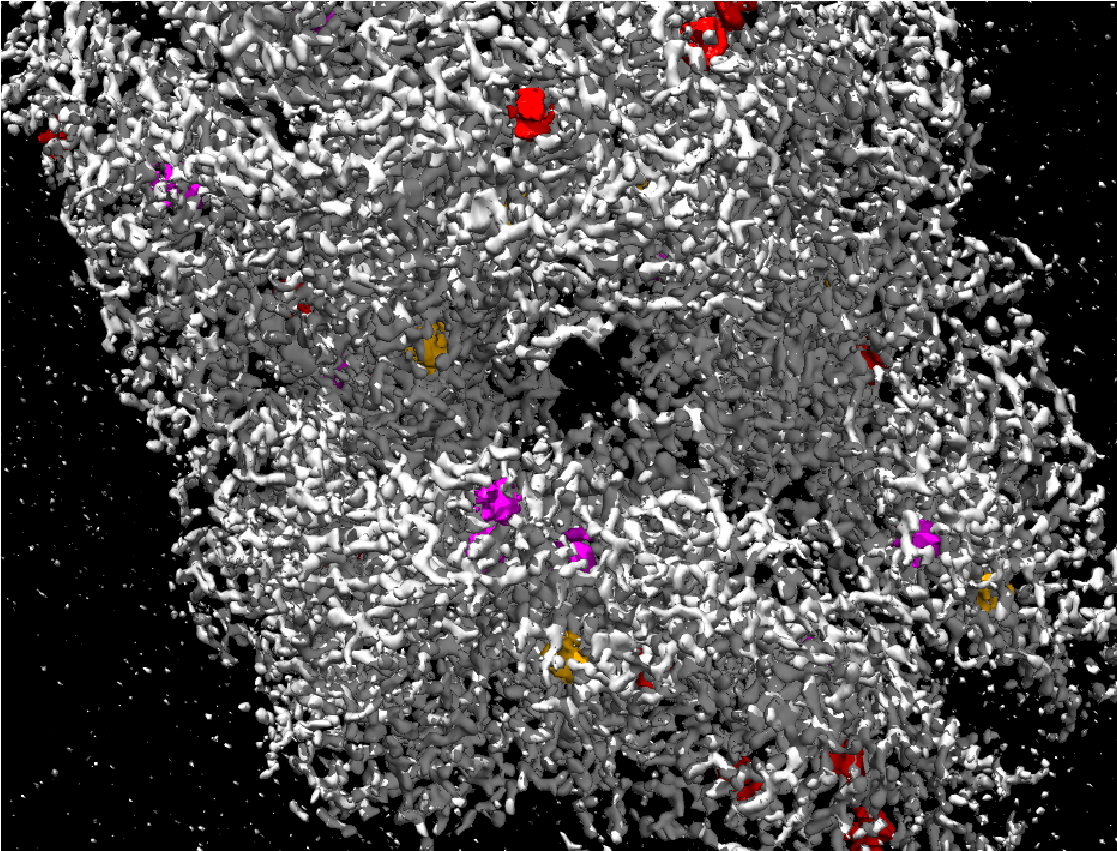
\includegraphics[scale = 0.14]{pics/res22.png} & 
      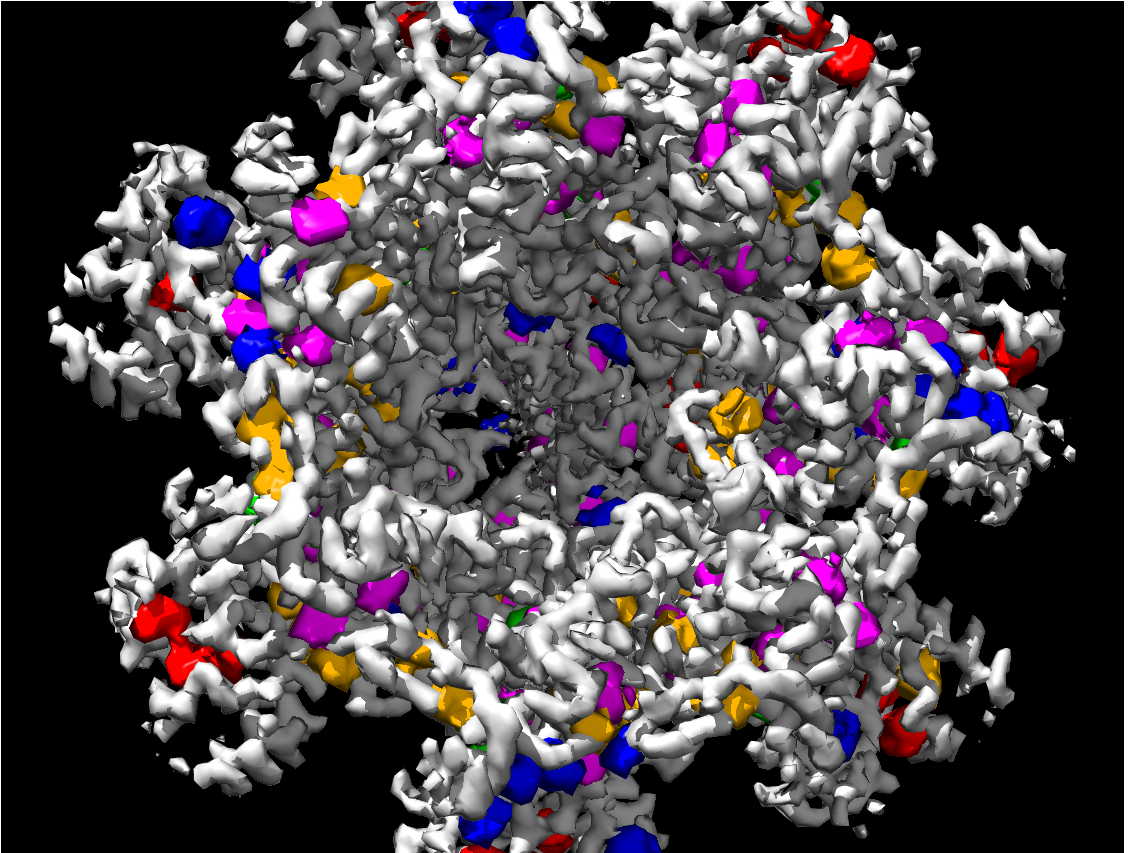
\includegraphics[scale = 0.14]{pics/res28.png} &
      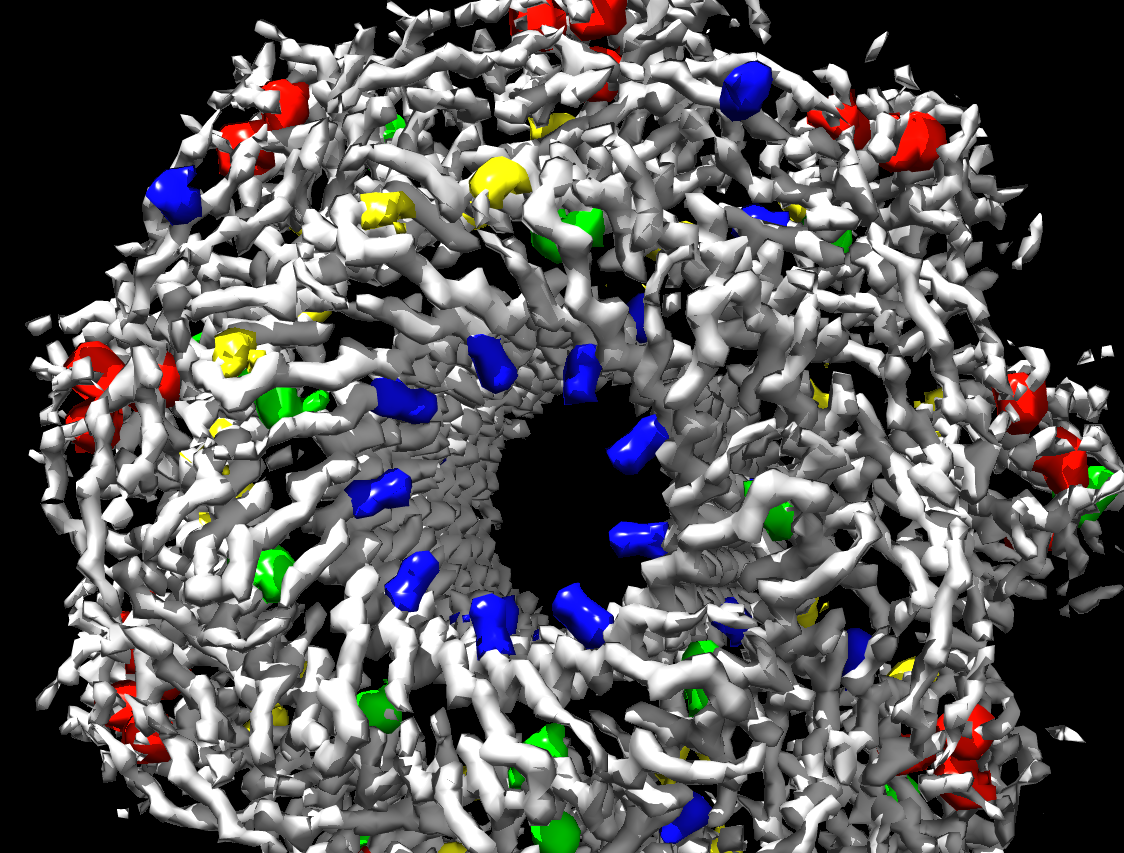
\includegraphics[scale = 0.14]{pics/lys_pore_GLY_LEU_LYS_TYR.png} \\
      \hline
      \color{black} ASN:----- 
      &
      \color{black} ASN: 5 out of 287 
      &
      \color{black} ASN: :-----   \\
      
      \color{black} ARG: 17 out of 133 
      &
      \color{black} ARG: 20 out of 119 
      &
      \color{black} ARG: 10 out of 117  \\

      \color{yellow} GLY: ----- 
      &
      \color{yellow} GLY: ----- 
      &
      \color{yellow} GLY: 25 out of 207  \\
      
      \color{red} LEU: 15 out of 231 
      &
      \color{red} LEU: 40 out of 231 
      &
      \color{red} LEU: 25 out of 108  \\
      
      \color{blue} LYS: ----- 
      &
      \color{blue} LYS: 30 out of 189 
      &
      \color{blue} LYS: 20 out of 171  \\

      \color{magenta} PRO: 10 out of 189 
      &
      \color{magenta} PRO: 80 out of 133 
      &
      \color{magenta} PRO: 9 out of 72  \\

      \color{green} TYR: ----- 
      &
      \color{green} TYR: 18 out of 91 
      &
      \color{green} TYR: 18 out of 144  \\

      \color{orange} VAL: 10 out of 119 
      &
      \color{orange} VAL: 35 out of 161 
      &
      \color{orange} VAL: -----  \\

      \hline

\end{tabular}
\caption{AANchor detection results for resolutions $2.2$ {\AA}  , $2.9$ {\AA} , and $3.1$ {\AA} } \label{t31}
\vspace{-3mm}
\end{table}

